\documentclass{article}

% Set page margin
% http://kb.mit.edu/confluence/pages/viewpage.action?pageId=3907057
\usepackage[margin=2.5cm]{geometry}

% Plots
\usepackage{pgfplots}

% Math operations
\usepackage{amsmath}

% FloatBarrier
\usepackage{placeins}

% Insert images from file path
\usepackage{graphicx}
\usepackage{wrapfig}

\usepackage{caption}

% Mono spaced font
\usepackage{bera}

% Referencing figures, listings etc. 
\usepackage{hyperref}
\usepackage{capt-of}

% Quotes
\usepackage{csquotes}

% some color definitions
\usepackage{xcolor}
\definecolor{cblue}{RGB}{16,78,139}
\definecolor{cred}{RGB}{139,37,0}
\definecolor{cgreen}{RGB}{0,139,0} 
\definecolor{corange}{RGB}{255,160,77}
\definecolor{clightblue}{RGB}{62,137,190}

% normal box
\newcommand{\sqboxs}{1.2ex}% the square size
\newcommand{\sqboxf}{0.6pt}% the border in \sqboxEmpty
\newcommand{\sqbox}[1]{\textcolor{#1}{\rule{\sqboxs}{\sqboxs}}}

% Code highlighting
\usepackage{color}
\usepackage{listings}
\usepackage{setspace}

% Define colors for Python listings
\definecolor{Code}{rgb}{0,0,0}
\definecolor{Decorators}{rgb}{0.5,0.5,0.5}
\definecolor{Numbers}{rgb}{0.5,0,0}
\definecolor{MatchingBrackets}{rgb}{0.25,0.5,0.5}
\definecolor{Keywords}{rgb}{0,0,1}
\definecolor{self}{rgb}{0,0,0}
\definecolor{Strings}{rgb}{0,0.63,0}
\definecolor{Comments}{rgb}{0,0.63,1}
\definecolor{Backquotes}{rgb}{0,0,0}
\definecolor{Classname}{rgb}{0,0,0}
\definecolor{FunctionName}{rgb}{0,0,0}
\definecolor{Operators}{rgb}{0,0,0}
\definecolor{Background}{rgb}{0.92,0.92,0.92}

\lstdefinelanguage{Python}{
	numbers=left,
	numberstyle=\footnotesize,
	numbersep=1em,
	xleftmargin=2em,
	framextopmargin=2em,
	framexbottommargin=2em,
	showspaces=false,
	showtabs=false,
	showstringspaces=false,
	frame=l,
	tabsize=4,
	% Basic
	basicstyle=\ttfamily\small\setstretch{1},
	backgroundcolor=\color{Background},
	% Comments
	commentstyle=\color{Comments}\slshape,
	% Strings
	stringstyle=\color{Strings},
	morecomment=[s][\color{Strings}]{"""}{"""},
	morecomment=[s][\color{Strings}]{'''}{'''},
	% keywords
	morekeywords={import,from,class,def,for,while,if,is,in,elif,else,not,and,or,print,break,continue,return,True,False,None,access,as,,del,except,exec,finally,global,import,lambda,pass,print,raise,try,assert},
	keywordstyle={\color{Keywords}\bfseries},
	% additional keywords
	morekeywords={[2]@invariant,pylab,numpy,np,scipy},
	keywordstyle={[2]\color{Decorators}\slshape},
	emph={self},
	emphstyle={\color{self}\slshape},
	%
}
\linespread{1.3}


% Define new float types so that I can reference them with captionof from the capt-of package. 
% https://tex.stackexchange.com/questions/6157/floating-an-algorithm
% Could be helpful as well: https://tex.stackexchange.com/questions/115499/image-caption-within-newfloat
\usepackage{float}
\newfloat{MyListing}{t}{lop}
\newfloat{Enumerate}{t}{lop2}


\begin{titlepage}
	\title{Assignment 2 - Convolutional Neural Network\\
		{\large Course: \textit{Advanced Machine Learning}}}
	\date{\today}	
\end{titlepage}




\begin{document}
	
	\maketitle
	
	\section{Teammembers and Contributions}
	\label{sec:TeammembersAndContributions}
	
	\begin{itemize}
		\item \makebox[0.4\linewidth]{\textbf{Bernd Menia}, \hfill\textit{01316129}:} Report, Programming, Testing, Plots
		\item \makebox[0.4\linewidth]{\textbf{Maximilian Samsinger}, \hfill\textit{01115383}:} Main Programming, Testing
	\end{itemize}
	
	\noindent The difference in our contributions is because Bernd just only started working with Machine Learning, while Maximilian has already prior knowledge in the subject. Thus we worked together, but the main programming work for this assignment was done by Maximilian. \\
	\\
	%Apart from that due to the size of the code we will only list the most important parts and explain them in detail with the gathered results. 
	In this month's assignment we had to program the Mountain Car task, as initially described by Moore's PhD thesis in 1990 \cite{Moore90efficientmemory-based}. Though as for the actual implementation we used the github project from Senadhi as a basis \cite{MountainCar-v02018}. 
	%In contrast to the other assignments we don't have much code for this one, so we will show more of our code snippets in this report. 
	
	
	\section{Task i}
	\label{sec:Taski}
	%In the first task we were asked to calculate the action-value function approximation by directly using the states and actions as inputs. For this we first transform the initial state and action into a vector, initialize the weight vector with all 0's and then multiply the two as seen as in (action\_value()). \\
	%\\
	Before the algorithm starts the policy approximation some values have to be initialized. Our initial state gets reset by calling $state = env.reset()$. Similar to that the first action gets set to $0$, which corresponds to going left. The features get calculated by calling convert\_to\_features(). Depending on the task the flag $polynomial$ gets so that the function behaves as following: \textbf{Task i}, $polynomial = false$) Simply append the initial state with the first action and return it. \textbf{Task ii}, $polynomial = true$) Converts the state to a polynomial of degree max\_degree. However, we cap the degree of action at 1, since we cannot expect higher powers of action to deliver meaningful extra features. Hereby the actions can be $0$, $1$ or $2$, corresponding to \textit{go left}, \textit{do nothing} and \textit{go right} respectively.\\
	\\
	The main part of the code consists of 3 nested for-loops as seen in \autoref{fig:loops}. The only thing the outermost loop does is to completely run the code n times. This was just done for convenience so that Task iii can be done without having to manually restart the program. The two inner loops are more interesting: The middle loop represents each episode of the algorithm while the innermost loop represents the steps that are made in each generation. 
	
	\begin{figure}
		\caption{Main part of the program with 3 nested for loops}
		\label{fig:loops}
		\lstinputlisting[language=Python]{code/loops.py}
	\end{figure}
	
	\FloatBarrier
	
	\noindent At the start of each episode the middle loop chooses the action that gets used, depending on which action is most suitable (see $choose\_action()$). From the second episode onwards the action that gets used is chosen by the algorithm, depending on which action is most suitable (choose\_action()). This is done creating a random number and comparing it to a threshold, epsilon, which we set to $0.02$. In other words this means that in $2\%$ of all cases the algorithm performs a random action. This is done to ensure that even when the algorithm is shifting towards a certain policy and is therefore almost fixed in its actions, there is still the possibility that it performs random actions which might lead to better results. The percentage is purposely low so that the actions still get mainly chosen by the best action calculated. The action also gets chosen anew in each step of each episode (innermost loop). 
	
	
	
	%At the start of each episode the middle loop decides with which values the weights should get initialized like described previously. 
	
	 %which can be seeen in a call to convert\_to\_features(). 
	%Regarding task 1 this function simply appends the starting state
	%randomly chooses the weights, ranging from 
	
	%The main part of the code consists of 2 nested for-loops. The outer loop represents each episode of the algorithm while the inner loop represents the steps that are made in each generation. The outer loop chooses the action that will get used to start the episode. At the start this action is dependant on the initially set values like described in the previous paragraph. \\
	%\\
	%From the second episode onwards the action that gets used is chosen by the algorithm, depending on which action is most suitable (choose\_action()). This is done creating a random number and comparing it to a threshold, epsilon, which we set to $0.02$. In other words this means that in $2\%$ of all cases the algorithm performs a random action. This is done to ensure that even when the algorithm is shifting towards a certain policy and is therefore almost fixed in its actions, there is still the possibility that it performs random actions which might lead to better results. The percentage is purposely low so that the actions still get mainly chosen by the best action calculated. The action gets chosen anew in each step of each episode. \\
	%\\
	
	\begin{figure}
		\caption{Choose an action with which the algorithm proceeds}
		\label{fig:chooseAction}
		\lstinputlisting[language=Python]{code/chooseAction.py}
	\end{figure}
	\newpage
	
	
	\noindent After an action has been chosen the algorithm performs a step. 
	%Hereby the actions can be $0$, $1$ or $2$, corresponding to \textit{go left}, \textit{do nothing} and \textit{go right} respectively. 
	The step also calculates the new state and the respective reward of the previous state in combination with the action.
	
	
	
	
	
	% Return or reward? 
	The reward gets calculated as follows: For each step that gets performed and after which the mountain car is not at the goal the reward is -1. On the contrary if after a step the goal got reached the reward is positive, though no exact numbers are given. \\
	\\
	The only thing left to do is to update the weights so that the policy gets approximated to the best possible values. As long as the goal hasn't been reached the weights get updated by taking into account the action\_value functions of the current- and previous states and also two not yet seen variables, learning\_rate and discount. The learning rate is used to decrease the amount of calculations that we have to make. Theoretically in order to get the best possible policy we would have to perform all combinations of sets and actions that exist. However this amount of complexity is not practical and cannot be achieved in a senseful manner. So instead of trying out all combinations of states and actions we choose one as described in choose\_action() and then dampen the value of the chosen action by multiplying the outcome with the learning\_rate. \\
	\\
	The other variable is the discount factor. The discount also acts as a kind of dampening factor, but it is more general than the learning\_rate. The exact formula how weight update gets calculated can be seen in X. \\
	\\
	Unfortunately our code doesn't work as expected. Sometimes the mountain car gets to the goal, but more often that not it doesn't. We don't know exactly why this is the case and so far we haven't figured it out. Also even when it reaches the goal the algorithm seems to unlearn this solution and the following episodes appear to be random again, disregarding which actions got it to the goal in the former episode. 
	
	
	%the algorithm chooses the action which it calculated to be the best to start 
	%Initially the feature vector gets set like described in the previous paragraph. After the fir
	
	%The main loop calls updates the weights in each generation. 
	
	
	\section{Task ii}
	\label{sec:Taskii}
	This task is quite similar to the first one. The difference is that the weights get initialized differently. How this is done is already described in \autoref{sec:Taski}. Since we had some issues getting Task i to work we also had the same issues for Task ii. 
	
	
	\section{Task iii}
	Finally in this task we compare the results from Task i and Task ii. Uhm I don't know what to write here since we don't really have results to compare :see\_no\_evil:.
	
	\begin{figure}[h]
		\caption{Average reward per step}
		\label{fig:AverageReward}
		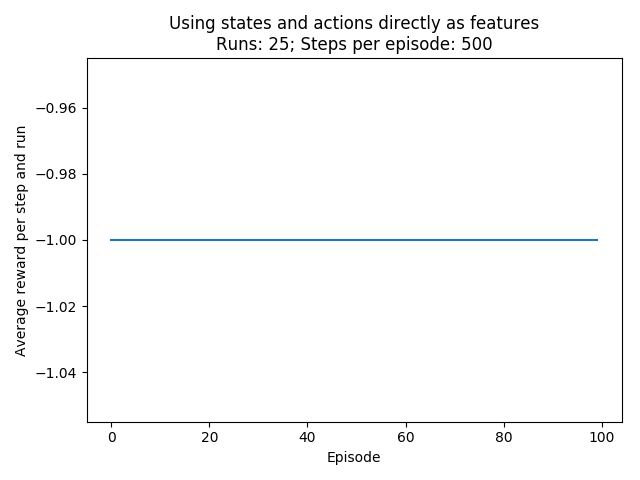
\includegraphics[width=0.9\textwidth]{plots/averageReward.png}
	\end{figure}
	
	
	\section{Discussion}
	As we have seen we ran into some problems while working on this assignment. First of all using polynomials as the initial values to approximate the action-value function is not good because it is highly likely that these values differ vastly from the actual underlying function that we try to approximate. Of course this is partly inevitable because by definition we don't know the underlying function yet and therefore have to approximate it. But there are far better methods to start the approximation, for example by using a Neural Network at first and then transferring the output to the Reinforcement Algorithms as the input, which is also the process that was used to train AlphaGo. 
	%Broadly spoken this is exactly what AlphaGo does. \\
	\\
	Another thing to mention is that our algorithm is unstable. Even after letting the algorithm run for 1000+ episodes the results from the episodes vary strongly as seen by the graph in X. Unfortunately we don't know why this is the case. \\
	\\
	Finally the major problem in our code is that our algorithm is prone to unlearning previously learned solutions. It may happen that it discovers a good way to drive upon the mountain, but the solution gets overwritten by the next episodes and therefore unlearns what brought it to the goal. 
	
	
	% Action 0² = 0, 1² = 1, 2² = 4 --> massive bias on moving right; encode in weight in action 
	
	\bibliographystyle{alpha}
	\bibliography{bibliography}
	
\end{document}